\begin{block}{Weak Scaling}
  \vspace{-0.5ex}
\begin{alertblock}{\textbf{MPI}}
\begin{figure}
    \centering
    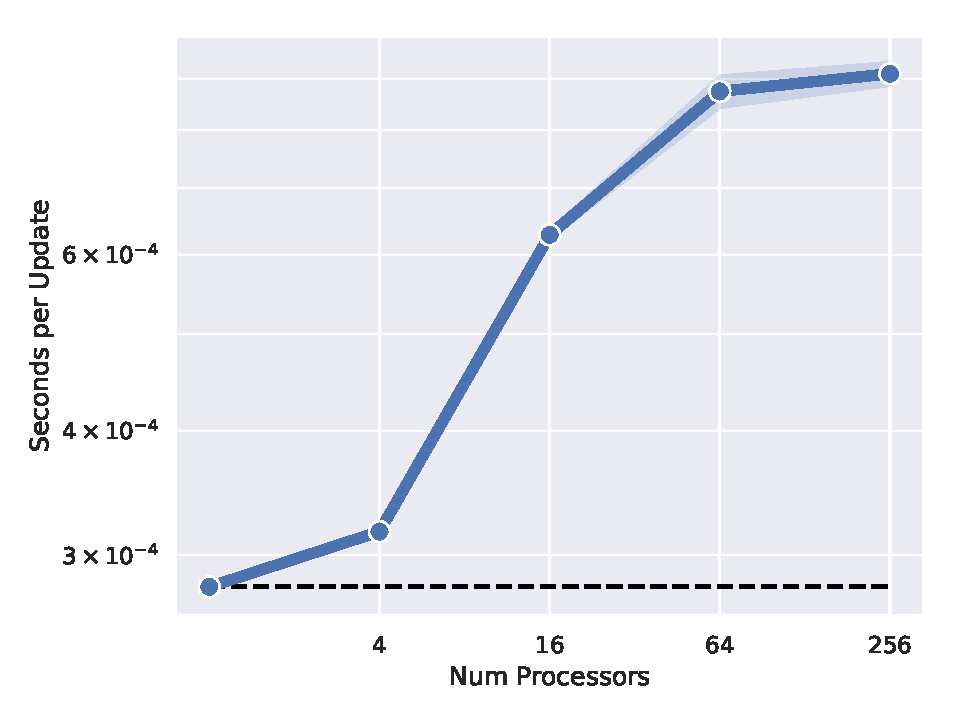
\includegraphics[width=0.9\textwidth]{img/MPIWeak}
  	\caption{
    Charm++ implementation time to solution versus parallelism for problem size proportional to CPU count (262,144 grid tiles per CPU).
    Dashed line indicates the ideal scaling relationship.
    Shaded area represents standard deviation of five replications for each observation.
    }
\end{figure}
\end{alertblock}
\vspace{-0.5ex}
\begin{alertblock}{\textbf{Charm++}}
\begin{figure}
    \centering
    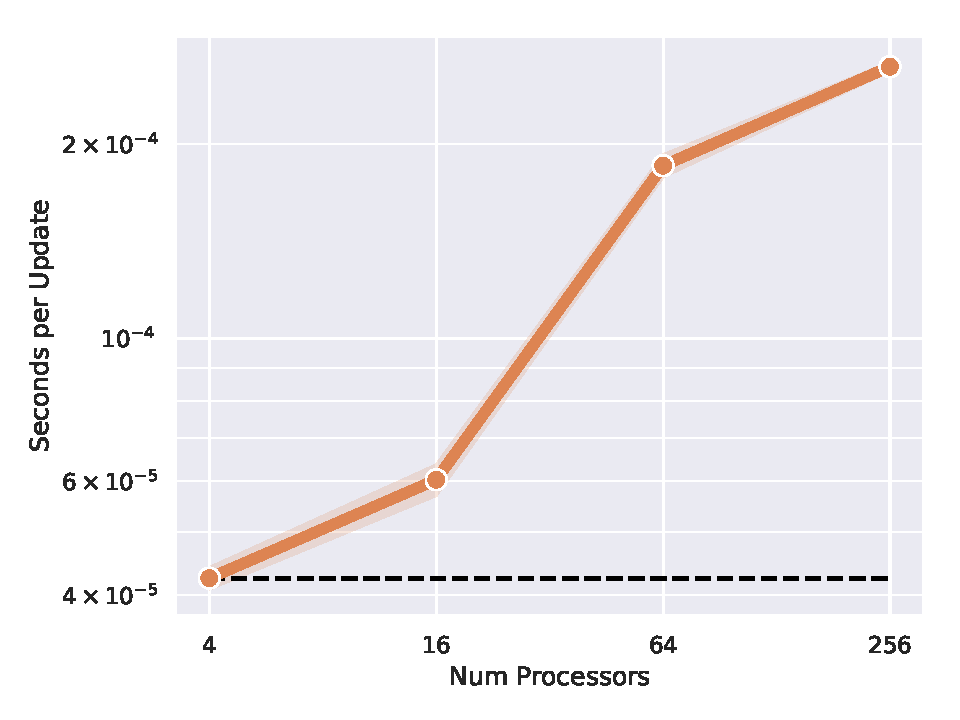
\includegraphics[width=\textwidth]{img/CharmWeak}
  	\caption{
    Charm++ implementation time to solution versus parallelism for problem size proportional to CPU count (1 grid tile per CPU).
    Dashed line indicates the ideal scaling relationship.
    Shaded area represents standard deviation of five replications for each observation.
    }
\end{figure}
\end{alertblock}

\end{block}
